\newpage
\section{Badania i~wyniki}

\subsection{Zbiór danych}

Badania przeprowadzono na czterech parach tokenów (WETH/USDC, WETH/USDT, WETH/DAI, WBTC/WETH), po
jednej puli na każdej z~dwóch giełd, w~czterech dwutygodniowych oknach obejmujących okresy
gwałtownych ruchów cen (tab.~\ref{tab:windows}). Pokrycie danymi każdej z~32 kombinacji pula--okno
wynosi 100\,\% bloków okna (\texttt{results/coverage.csv}). Łącznie baza zawiera 250\,373 bloki
z~metadanymi, 795\,618 zdarzeń \texttt{Sync}, 786\,828 zdarzeń \texttt{Swap} i~1\,418\,144 stany
par w~blokach. Rozbieżność powyżej progu $0{,}65\,\%$ wystąpiła w~4\,829 blokach, co stanowi
$0{,}34\,\%$ wszystkich stanów; wszystkie te okazje poddano weryfikacji retrospektywnej.

\begin{table}[H]\centering\small
\caption{Okna analizy i~liczności (cztery pary łącznie)}\label{tab:windows}
\begin{tabular}{llrrrr}
\toprule
Okno & Daty (UTC) & Bloki & Stany par & Okazje & Okazje/stany \\
\midrule
2021-05 krach & 14--26.05.2021 & 12\,429\,199--12\,506\,592 & 309\,548 & 2\,236 & 0{,}72\,\% \\
2021-11 ATH   & 05--19.11.2021 & 13\,553\,257--13\,642\,393 & 356\,441 & 891   & 0{,}25\,\% \\
2022-05 Luna  & 05--19.05.2022 & 14\,713\,964--14\,801\,795 & 351\,295 & 1\,296 & 0{,}37\,\% \\
2022-11 FTX   & 05--19.11.2022 & 15\,900\,096--16\,000\,337 & 400\,860 & 406   & 0{,}10\,\% \\
\bottomrule
\end{tabular}
\end{table}

Wynik weryfikacji retrospektywnej zestawia tabela~\ref{tab:verif}. Status
\texttt{consumed\_atomic} otrzymało 714 okazji, z~czego 570 o~trasie \texttt{two\_pool}
i~144 o~trasie \texttt{multi} (wykluczone z~populacji ewaluacji). Etykietę pozytywną
(\texttt{profitable\_consumed}) ma 544 okazji, czyli $11{,}6\,\%$ populacji o~znanej etykiecie
($n=4\,685$). Udział konsumpcji atomowych jest najwyższy w~oknie 2021-05 (27,6\,\% okazji). W~trzech
późniejszych oknach wynosi już tylko 2,7--4,6\,\%, a~w~oknie 2022-11 dla par WETH/DAI
i~WBTC/WETH nie zarejestrowano ani jednej. Rozkład opóźnienia konsumpcji dla trasy
\texttt{two\_pool} przedstawia rys.~\ref{fig:khist}: 124 okazje ($21{,}8\,\%$) skonsumowano
w~tym samym bloku, 247 w~następnym, a~90 ($15{,}8\,\%$) dopiero w~trzecim bloku po wykryciu.
Liczby dotyczą okazji, nie transakcji. Rozbieżność, która utrzymuje się przez kilka bloków, jest
osobną okazją w~każdym z~nich, a~zamyka ją zwykle ta sama transakcja, dlatego za 570 konsumpcji
\texttt{two\_pool} odpowiada 345 różnych transakcji.

\begin{table}[H]\centering\footnotesize
\caption{Statusy weryfikacji retrospektywnej według okien (cztery pary łącznie);
  \texttt{gas=0} --- konsumpcje z~zerową ceną gazu (pakiety MEV)}\label{tab:verif}
\begin{tabular}{lrrrrrrrr}
\toprule
Okno & Okazje & atomic & \ \ gas=0 & partial & decayed & persisted & two\_pool & multi \\
\midrule
2021-05 krach & 2\,236 & 618 & 131 & 1\,390 & 18 & 210 & 500 & 118 \\
2021-11 ATH   & 891   & 25  & 0   & 417   & 2  & 447 & 20  & 5   \\
2022-05 Luna  & 1\,296 & 60  & 0   & 804   & 20 & 412 & 43  & 17  \\
2022-11 FTX   & 406   & 11  & 0   & 303   & 4  & 88  & 7   & 4   \\
\midrule
razem         & 4\,829 & 714 & 131 & 2\,914 & 44 & 1\,157 & 570 & 144 \\
\bottomrule
\end{tabular}
\end{table}

Tabela~\ref{tab:features-label} zestawia mediany cech w~populacji ewaluacji według okien i~etykiety oraz
nasycenie dziedzin cech $G$ i~$L$ we wszystkich stanach bloków okna. W~oknie 2021-05 dla par
WETH/USDC, WETH/USDT i~WBTC/WETH cecha $L$ osiąga górną granicę dziedziny (100~mln USD) w~każdym
bloku okna, dla WETH/DAI w~80,6\,\% bloków.

\begin{table}[H]\centering\scriptsize\setlength{\tabcolsep}{3pt}
\caption{Mediany cech w~populacji ewaluacji według okien i~etykiety ($+$ --- zyskownie skonsumowane,
  $-$ --- pozostałe) oraz udział stanów bloków okna z~$L=100$ (górna granica dziedziny)
  i~$G\ge0{,}6$ (dolna granica termu ,,zaporowy'')}\label{tab:features-label}
\begin{tabular}{lrrrrrrrrrrrr}
\toprule
 & \multicolumn{2}{c}{$n$} & \multicolumn{2}{c}{$S$ [\%]} & \multicolumn{2}{c}{$G$ [\%]} & \multicolumn{2}{c}{$L$ [mln USD]} & \multicolumn{2}{c}{$M$} & \multicolumn{2}{c}{bloki okna [\%]} \\
\cmidrule(lr){2-3}\cmidrule(lr){4-5}\cmidrule(lr){6-7}\cmidrule(lr){8-9}\cmidrule(lr){10-11}\cmidrule(lr){12-13}
Okno & $+$ & $-$ & $+$ & $-$ & $+$ & $-$ & $+$ & $-$ & $+$ & $-$ & $L{=}100$ & $G{\ge}0{,}6$ \\
\midrule
2021-05 krach & 477 & 1\,641 & 0{,}972 & 0{,}781 & 0{,}590 & 0{,}345 & 100{,}0 & 100{,}0 & 95{,}6 & 90{,}3 & 95{,}2 & 1{,}2 \\
2021-11 ATH   & 20  & 866    & 0{,}854 & 0{,}697 & 0{,}283 & 0{,}266 & 100{,}0 & 100{,}0 & 81{,}1 & 69{,}8 & 75{,}0 & 0{,}6 \\
2022-05 Luna  & 40  & 1\,239 & 1{,}232 & 0{,}784 & 0{,}218 & 0{,}237 & 40{,}9  & 19{,}3  & 96{,}5 & 94{,}3 & 25{,}0 & 0{,}1 \\
2022-11 FTX   & 7   & 395    & 1{,}104 & 0{,}756 & 0{,}034 & 0{,}041 & 23{,}6  & 7{,}9   & 97{,}2 & 93{,}8 & 0{,}0  & 0{,}0 \\
\bottomrule
\end{tabular}
\end{table}

\begin{figure}[H]\centering
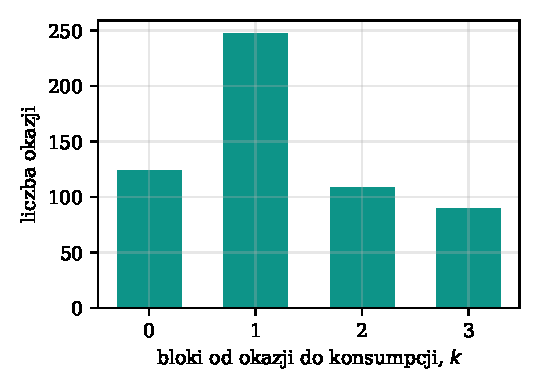
\includegraphics[width=.5\linewidth]{Images/k-hist.pdf}
\caption{Liczba bloków od wykrycia okazji do transakcji konsumującej (trasa \texttt{two\_pool};
  $n=570$ okazji zamkniętych przez 345 transakcji)}
\label{fig:khist}
\end{figure}

\subsection{Protokół ewaluacji}

Wszystkie metryki porównawcze liczone są na populacji zweryfikowanych okazji o~znanej etykiecie:
\texttt{opportunity\_verifications} złączone z~\texttt{opportunities}, z~wykluczeniem trasy
\texttt{multi} (ADR~0008). Osobna populacja wszystkich stanów bloków (tło jako klasa 0) jest
zapisywana wyłącznie diagnostycznie; odróżnienie okazji od tła jest na niej trywialne (AUC
$\approx 0{,}99$) i~nie służy do porównań.

Modele uczone na danych ocenia się w~podziale międzyoknowym: konfiguracja \emph{W2} trenuje na
oknie 2021-05 i~testuje na oknach 2021-11, 2022-05 i~2022-11; konfiguracja \emph{W2+W4}
(międzyreżimowa) trenuje na oknach 2021-05 i~2022-05, a~testuje na 2021-11 i~2022-11. Wewnątrz
treningu ANFIS 20\,\% grup służy do wczesnego zatrzymania. Grupą jest zbiór okazji dzielących
tę samą transakcję konsumującą, a~dla okazji bez transakcji klaster sąsiednich okazji tej samej
pary w~oknie (przerwa $\le 3$ bloki); tło to singletony (ADR~0007). Podział grupowy jest
konieczny, bo 198 zweryfikowanych konsumpcji atomowych w~oknie 2021-05 pochodzi tylko ze 129
transakcji.

Metryki podstawowe to AUC (statystyka Manna--Whitneya z~remisami liczonymi po 0,5) oraz PR-AUC
(średnia precyzja z~interpolacją krokową), obie niezależne od progu. Przy stałym progu
$\mathrm{score}\ge 50$ raportowane są precyzja, czułość i~$F_1$. Baseline~v2 ma próg dobrany na
etykietach okna kalibracji, a~pozostałe modele próg stały, dlatego dla każdego modelu podaje się
też próg F1-optymalny na jego oknach treningowych (ADR~0006). Przedział ufności 95\,\% dla AUC
pochodzi z~bootstrapu stratyfikowanego po klasie (1000 prób, ziarno 42, percentyle 2,5 i~97,5).
Stabilność ANFIS względem inicjalizacji i~tasowania oceniono na pięciu ziarnach (42--46) dla
każdej konfiguracji. Wszystkie liczby w~tym rozdziale generuje polecenie
\texttt{npm run export-results}, korzystające z~tych samych funkcji, które obsługują API.

\subsection{Poprawność implementacji}

\paragraph{Testy automatyczne.} Repozytorium zawiera 140 plików testowych z~953 przypadkami
(Vitest) w~czterech warstwach: jednostkowe (czyste funkcje), integracyjne z~bazą testową
(osobna baza z~sufiksem \texttt{\_test}, chroniona przed pomyleniem z~bazą roboczą), testy na
żywym węźle RPC (włączane zmienną środowiskową) oraz regresje względem danych referencyjnych.
Pokrycie linii wynosi 99,3\,\% dla pakietu \texttt{core} i~99,7\,\% dla \texttt{analysis} przy
progu 80\,\% wymuszanym w~konfiguracji; pozostałe pakiety mają pokrycie 94,7--100\,\%. Testy
arytmetyki AMM porównują \texttt{getAmountOut} z~kwotami rzeczywistych swapów z~łańcucha, testy
systemu Mamdaniego odtwarzają sześć scenariuszy i~rozkład etykiet implementacji referencyjnej,
a~testy
weryfikacji używają zapisanych paragonów transakcji, więc nie zależą od dostępności RPC. Potok
CI (GitHub Actions) uruchamia sprawdzenie typów, lint, migracje na usłudze PostgreSQL~16, testy
z~pokryciem i~budowę interfejsu przy każdym wypchnięciu na gałąź główną.

\paragraph{Niezmienniki danych.} Dwanaście ograniczeń \texttt{CHECK} dodano do schematu po
zebraniu danych; zapytania kontrolne przed ich włączeniem nie wykazały żadnego naruszenia na
1,4~mln stanów, 4\,829 okazjach i~23,2~mln ocen modeli.

\paragraph{Kontrola ręczna weryfikacji.} Heurystyki klasyfikacji (kandydat, beneficjent,
trasa) sprawdzono niezależnie od kodu, porównując wiersze
\texttt{opportunity\_verifications} z~odczytem tych samych transakcji w~serwisie Etherscan.
Próba objęła 10 pierwszych chronologicznie konsumpcji atomowych pary WETH/USDC w~oknie 2021-05
oraz 3 kontrole statusów \texttt{decayed}/\texttt{persisted}. Wyniki: 10/10 zgodnych co do
\texttt{gas\_used} (co do jednostki) i~kierunków swapów, 9/10 zgodnych co do znaku i~rzędu
wielkości zysku (2/10 z~dokładnością poniżej 1~USD), 1/10 poprawnie sklasyfikowana jako trasa
\texttt{multi} (agregator między pulami), 3/3 kontrole negatywne bez fałszywych negatywów.
Trzy transakcje z~zawijaniem i~odwijaniem WETH potwierdziły, że po korekcie ETH~$\equiv$~WETH
zysk zrealizowany zmienia się z~artefaktu rzędu 1,6~mln USD na 35,8~tys.~USD (szczegóły
w~\texttt{docs/verification-method.md}). Kontrolę można powtórzyć testem
\texttt{known-tx.test.ts} na żywym RPC.

\paragraph{Odtwarzalność.} Skrypt \texttt{scripts/reproduce.sh} odtwarza całość od pustej bazy:
64 zadania danych (mediana czasu pobrania puli w~oknie 334~s, analizy pary 10,5~s, weryfikacji
0,7~s), kalibrację baseline~v2 (28~s) i~10 treningów ANFIS (mediana 37~s). Każdy zapis modelu
niesie proweniencję: skrót commitu, wersje bibliotek, zakresy bloków i~liczności tabel
(\texttt{results/provenance.json}).

\subsection{Studium przypadku: droga jednej okazji}

Pozostałe podrozdziały podają metryki zagregowane po całej populacji. Poniżej prześledzono jedną okazję od stanu pul w~bloku
aż po etykietę weryfikacji, co pokazuje, jaką informację system daje o~pojedynczej
rozbieżności. Przypadek dobrano jako \emph{wzorcowy, a~nie typowy}:
rozbieżność jest duża, a~kolejne etapy przetwarzania dają zgodny rachunek, co pozwala zestawić
je obok siebie. Zastrzeżenia o~reprezentatywności zebrano na końcu podrozdziału.


\paragraph{Powstanie rozbieżności.} Okazja dotyczy pary WETH/USDC w~oknie 2021-05 i~obejmuje
cztery kolejne bloki (tab.~\ref{tab:case-blocks}). W~bloku 12\,430\,486 do puli Uniswapa trafiło
391,43~WETH w~zamian za 1\,466\,334,87~USDC; cena w~tej puli spadła zgodnie z~niezmiennikiem
$x\cdot y=k$, a~pula Sushiswapa pozostała bez zmian, bo nie zaszła w~niej wówczas żadna wymiana.
Rozbieżność utrzymała się przez jeden blok i~zamknęła w~bloku 12\,430\,488.

\begin{table}[H]\centering\small
\caption{Stan pary WETH/USDC w~czterech kolejnych blokach okna 2021-05 (ceny w~USDC za 1~WETH)}
\label{tab:case-blocks}
\begin{tabular}{rrrrl}
\toprule
Blok & Uniswap & Sushiswap & $S$ [\%] & Zdarzenie \\
\midrule
12\,430\,485 & 3\,791,00 & 3\,801,05 & 0,265 & stan poniżej progu \\
12\,430\,486 & 3\,723,96 & 3\,801,05 & 2,070 & sprzedaż 391,43 WETH w~Uniswapie \\
12\,430\,487 & 3\,724,57 & 3\,801,00 & 2,052 & \textbf{okazja omawiana poniżej} \\
12\,430\,488 & 3\,774,14 & 3\,777,82 & 0,097 & transakcja arbitrażowa domyka lukę \\
\bottomrule
\end{tabular}
\end{table}

\paragraph{Cechy i~wykrycie.} W~bloku 12\,430\,487 rozbieżność $S=2{,}052\,\%$ przekracza próg
0,65\,\%, więc blok trafia do tabeli \texttt{opportunities}. Pozostałe cechy wynoszą
$G=0{,}139\,\%$, $L=100{,}0$~mln~USD (górna granica dziedziny) i~$M=65{,}1$. Bazowy token jest
tańszy w~Uniswapie, więc kierunek to \texttt{a->b}. Optymalna wielkość transakcji policzona
wzorem z~fragmentu~\ref{lst:opttrade} wynosi 664\,266,81~USDC i~daje zysk brutto 4\,767,91~USD;
po odjęciu szacowanego kosztu gazu 69,65~USD (220\,000 jednostek przy medianie 85~gwei w~tym
bloku) zysk netto wynosi 4\,698,26~USD.

\paragraph{Oceny modeli.} Tę samą okazję cztery modele oceniają różnie
(tab.~\ref{tab:case-scores}). System Mamdaniego uruchamia dokładnie dwie reguły: R11 z~siłą
0,245 (konkluzja ,,wykonalna'') i~R13 z~siłą 0,255 (konkluzja ,,ryzykowna''), a~centroid
agregatu wypada między nimi. Warto odróżnić ocenę od etykiety słownej: próg klasyfikacji
binarnej wynosi 50, więc ocena 52,25 jest predykcją pozytywną, mimo że etykieta wyznaczona
z~funkcji przynależności $W$ brzmi ,,ryzykowna''.

\begin{table}[H]\centering\small
\caption{Oceny okazji z~bloku 12\,430\,487 wystawione przez cztery modele}
\label{tab:case-scores}
\begin{tabular}{llr l}
\toprule
Model & Ocena & & Etykieta \\
\midrule
baseline v1      & 70,73  & & wykonalna \\
Mamdani          & 52,25  & & ryzykowna \\
baseline v2      & 100,00 & & atrakcyjna \\
ANFIS W2+W4      & 88,50  & & atrakcyjna \\
\bottomrule
\end{tabular}
\end{table}

\paragraph{Weryfikacja retrospektywna.} W~bloku bezpośrednio następującym ($k=1$) system
odnajduje transakcję \texttt{0xe2991cbb\ldots eafc46be} o~trasie dwupulowej, która zamyka
rozbieżność. Zysk zrealizowany brutto wynosi 4\,776,76~USD, zużycie gazu 97\,344 jednostki
o~koszcie 553,19~USD, a~zysk netto 4\,223,57~USD, więc etykieta
\texttt{profitable\_consumed} przyjmuje wartość prawda. Komplet tych informacji --- cechy,
aktywacje reguł, oceny modeli i~wynik weryfikacji wraz z~odnośnikiem do eksploratora łańcucha
--- interfejs pokazuje w~panelu szczegółów okazji (rys.~\ref{fig:ui-okazja}).

\begin{figure}[H]\centering
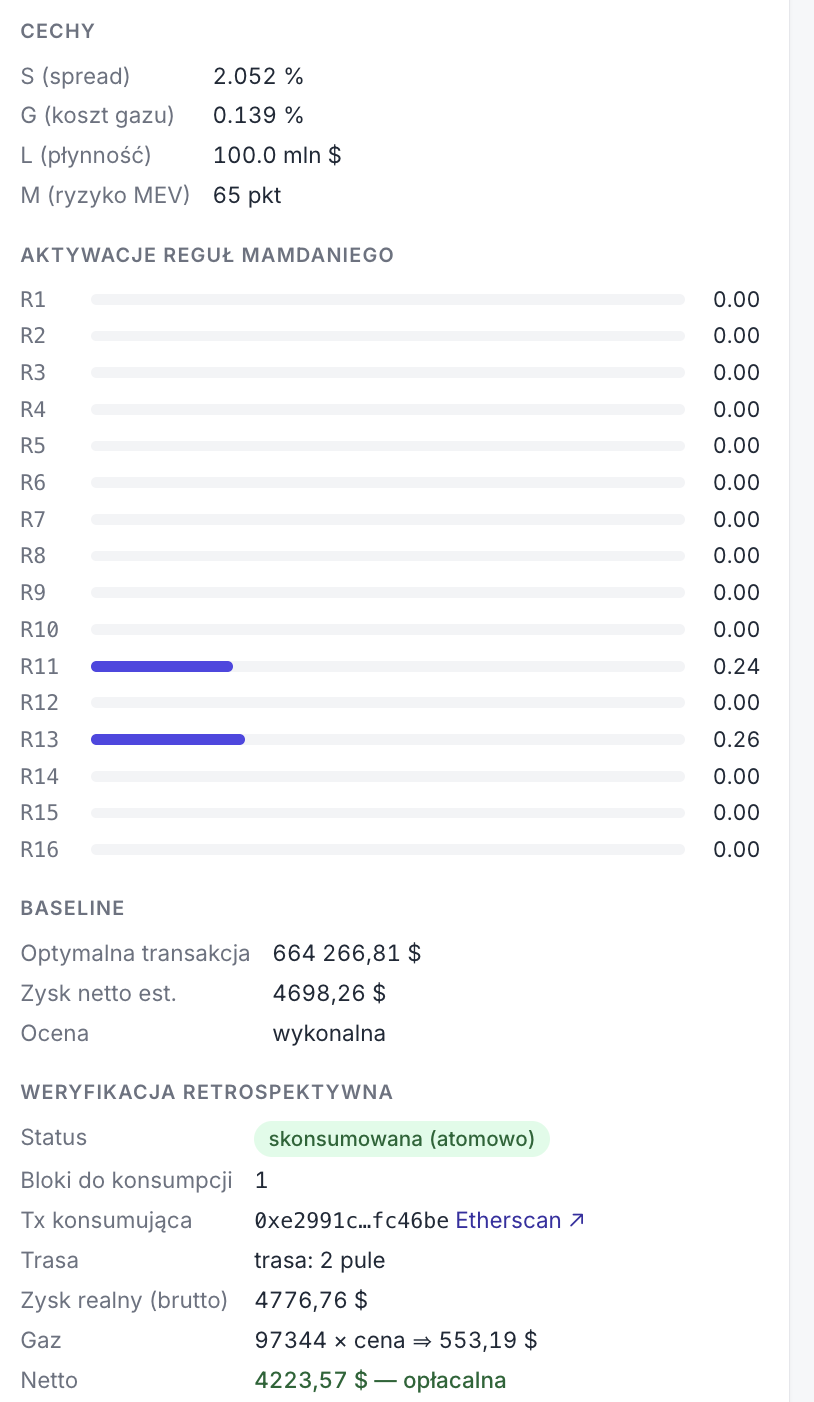
\includegraphics[width=.46\linewidth]{Images/ui-okazja-szczegoly.png}
\caption{Panel szczegółów okazji: cechy, aktywacje 16 reguł systemu Mamdaniego, wynik
heurystyki oraz weryfikacja retrospektywna (zrzut ekranu)}\label{fig:ui-okazja}
\end{figure}

\paragraph{Wnioski z~przypadku.} Szacunek zysku brutto (4\,767,91~USD) różni się od wartości
zrealizowanej (4\,776,76~USD) o~0,19\,\%, co potwierdza poprawność arytmetyki puli. Cała
istotna rozbieżność leży natomiast po stronie kosztu: szacunek zakłada medianę ceny gazu
w~bloku i~daje 69,65~USD, podczas gdy zwycięzca zapłacił 553,19~USD, czyli blisko ośmiokrotnie
więcej, ponieważ o~kolejność w~bloku konkuruje się właśnie ceną gazu. Dokładny jest zatem model
wyceny, a~nie model kosztu --- obserwacja ta wraca w~podrozdziale~4.8.

Przypadek jest wzorcowy i~nie należy go uogólniać: rozbieżność 2\,\% mieści się w~górnym
ogonie rozkładu, a~oceny wszystkich czterech modeli są tu zgodne co do kierunku. W~populacji
takiej zgodności nie ma --- porównanie modeli w~kolejnym podrozdziale pokazuje, że przewaga
jednego nad drugim jest kwestią kilku punktów AUC, a~nie pojedynczych trafień.

\subsection{Porównanie modeli}

Tabela~\ref{tab:models} zestawia pięć modeli: baseline~v1, system Mamdaniego, baseline~v2
(kalibrowany na oknie 2021-05) oraz ANFIS w~dwóch konfiguracjach (ziarno 42). Wiersze oznaczone
,,(tr)'' dotyczą okien użytych do treningu lub kalibracji danego modelu i~nie są miarą
generalizacji. Krzywe ROC dla wszystkich okien łącznie pokazuje rys.~\ref{fig:rocall},
a~w~podziale na okna rys.~\ref{fig:rocwin}. Pełna tabela dla wszystkich 19 modeli, w~tym
historycznych, znajduje się w~pliku \texttt{results/evaluation.md}.

\begin{table}[H]\centering\scriptsize\setlength{\tabcolsep}{3.5pt}
\caption{Metryki modeli na populacji zweryfikowanych okazji ($n$ --- liczność, $n_+$ --- pozytywy;
  próg 50; ,,(tr)'' --- okno treningowe/kalibracyjne modelu)}\label{tab:models}
\begin{tabular}{llrrrrrrl}
\toprule
Okno & Model & $n$ & $n_+$ & Prec. & Czułość & $F_1$ & PR-AUC & AUC [95\,\% CI] \\
\midrule
2021-05 krach & baseline v1  & 2118 & 477 & 0{,}536 & 0{,}109 & 0{,}181 & 0{,}331 & 0{,}627 [0{,}60--0{,}65] \\
 & Mamdani      & 2118 & 477 & 0{,}222 & 0{,}017 & 0{,}031 & 0{,}197 & 0{,}392 [0{,}36--0{,}42] \\
 & baseline v2 (tr) & 2118 & 477 & 0{,}350 & 0{,}706 & 0{,}468 & 0{,}397 & 0{,}700 [0{,}67--0{,}72] \\
 & ANFIS W2 (tr) & 2118 & 477 & 0{,}246 & 0{,}975 & 0{,}393 & 0{,}426 & 0{,}712 [0{,}69--0{,}74] \\
 & ANFIS W2+W4 (tr) & 2118 & 477 & 0{,}228 & 0{,}994 & 0{,}370 & 0{,}415 & 0{,}707 [0{,}68--0{,}73] \\
\midrule
2021-11 ATH & baseline v1  & 886 & 20 & 0{,}000 & 0{,}000 & 0{,}000 & 0{,}038 & 0{,}599 [0{,}51--0{,}70] \\
 & Mamdani      & 886 & 20 & 0{,}000 & 0{,}000 & 0{,}000 & 0{,}017 & 0{,}359 [0{,}25--0{,}46] \\
 & baseline v2  & 886 & 20 & 0{,}153 & 0{,}650 & 0{,}248 & 0{,}107 & 0{,}825 [0{,}74--0{,}90] \\
 & ANFIS W2     & 886 & 20 & 0{,}029 & 0{,}850 & 0{,}056 & 0{,}073 & 0{,}737 [0{,}62--0{,}85] \\
 & ANFIS W2+W4  & 886 & 20 & 0{,}023 & 1{,}000 & 0{,}045 & 0{,}100 & 0{,}762 [0{,}64--0{,}87] \\
\midrule
2022-05 Luna & baseline v1  & 1279 & 40 & 0{,}175 & 0{,}175 & 0{,}175 & 0{,}107 & 0{,}713 [0{,}63--0{,}79] \\
 & Mamdani      & 1279 & 40 & 0{,}000 & 0{,}000 & 0{,}000 & 0{,}039 & 0{,}593 [0{,}52--0{,}67] \\
 & baseline v2  & 1279 & 40 & 0{,}098 & 0{,}575 & 0{,}168 & 0{,}138 & 0{,}800 [0{,}72--0{,}87] \\
 & ANFIS W2     & 1279 & 40 & 0{,}045 & 0{,}250 & 0{,}077 & 0{,}055 & 0{,}702 [0{,}63--0{,}76] \\
 & ANFIS W2+W4 (tr) & 1279 & 40 & 0{,}081 & 0{,}600 & 0{,}142 & 0{,}137 & 0{,}778 [0{,}71--0{,}84] \\
\midrule
2022-11 FTX & baseline v1  & 402 & 7 & 0{,}125 & 0{,}286 & 0{,}174 & 0{,}097 & 0{,}788 [0{,}61--0{,}95] \\
 & Mamdani      & 402 & 7 & 0{,}000 & 0{,}000 & 0{,}000 & 0{,}037 & 0{,}731 [0{,}61--0{,}84] \\
 & baseline v2  & 402 & 7 & 0{,}071 & 0{,}286 & 0{,}114 & 0{,}128 & 0{,}839 [0{,}70--0{,}95] \\
 & ANFIS W2     & 402 & 7 & 0{,}000 & 0{,}000 & 0{,}000 & 0{,}032 & 0{,}677 [0{,}50--0{,}82] \\
 & ANFIS W2+W4  & 402 & 7 & 0{,}087 & 0{,}286 & 0{,}133 & 0{,}126 & 0{,}879 [0{,}79--0{,}95] \\
\midrule
wszystkie okna & baseline v1  & 4685 & 544 & 0{,}370 & 0{,}112 & 0{,}172 & 0{,}210 & 0{,}654 [0{,}63--0{,}68] \\
 & Mamdani      & 4685 & 544 & 0{,}101 & 0{,}015 & 0{,}026 & 0{,}097 & 0{,}354 [0{,}33--0{,}38] \\
 & baseline v2  & 4685 & 544 & 0{,}286 & 0{,}689 & 0{,}405 & 0{,}326 & 0{,}796 [0{,}78--0{,}81] \\
 & ANFIS W2     & 4685 & 544 & 0{,}180 & 0{,}904 & 0{,}300 & 0{,}269 & 0{,}787 [0{,}77--0{,}81] \\
 & ANFIS W2+W4  & 4685 & 544 & 0{,}159 & 0{,}956 & 0{,}273 & 0{,}369 & 0{,}818 [0{,}80--0{,}83] \\
\bottomrule
\end{tabular}
\end{table}

Progi F1-optymalne wyznaczone na oknach treningowych wynoszą 50,0 dla baseline~v2 (z~konstrukcji),
80,4 dla ANFIS~W2 i~81,5 dla ANFIS~W2+W4; oba modele ANFIS przy progu 50 klasyfikują jako
pozytywne 58--70\,\% populacji, co widać w~wysokiej czułości i~niskiej precyzji w~tabeli.
Kalibracja baseline~v2 wybrała z~siatki 30 kombinacji punkt $\mathrm{gasUnits}=150\,000$,
$\kappa=0$, $w=0$ (próg $v=0{,}728$, skala 70,6), czyli ranking okazji według samego zysku brutto;
sąsiednie punkty siatki z~$\kappa=0{,}25$ miały AUC niższe o~0,01--0,04 na oknie kalibracji.

Wiersz ,,wszystkie okna'' łączy okna testowe z~treningowymi: dla baseline~v2 i~ANFIS~W2 okno
kalibracji lub treningu 2021-05 stanowi 45,2\,\% populacji (2\,118 z~4\,685), dla ANFIS~W2+W4 okna
2021-05 i~2022-05 stanowią 72,5\,\% (3\,397 z~4\,685); baseline~v1 i~Mamdani nie mają okien
treningowych. Miarą generalizacji są więc wyłącznie wiersze okien testowych.

\begin{figure}[H]\centering
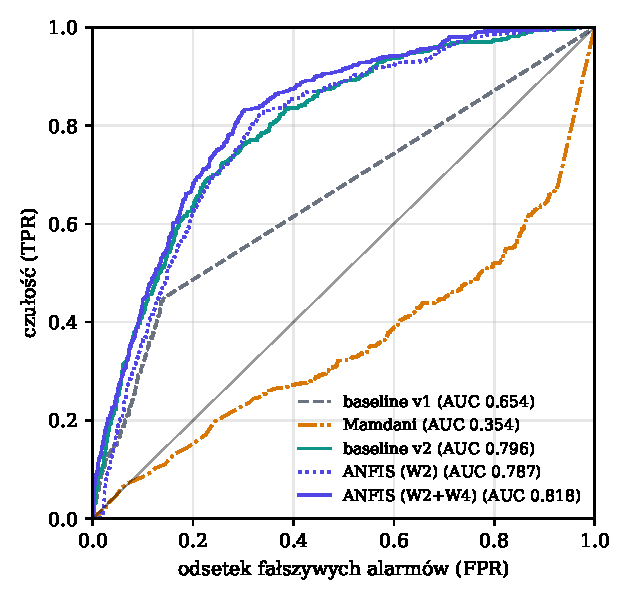
\includegraphics[width=.62\linewidth]{Images/roc-all.pdf}
\caption{Krzywe ROC pięciu modeli na wszystkich oknach łącznie ($n=4\,685$, $n_+=544$)}
\label{fig:rocall}
\end{figure}

\begin{figure}[H]\centering
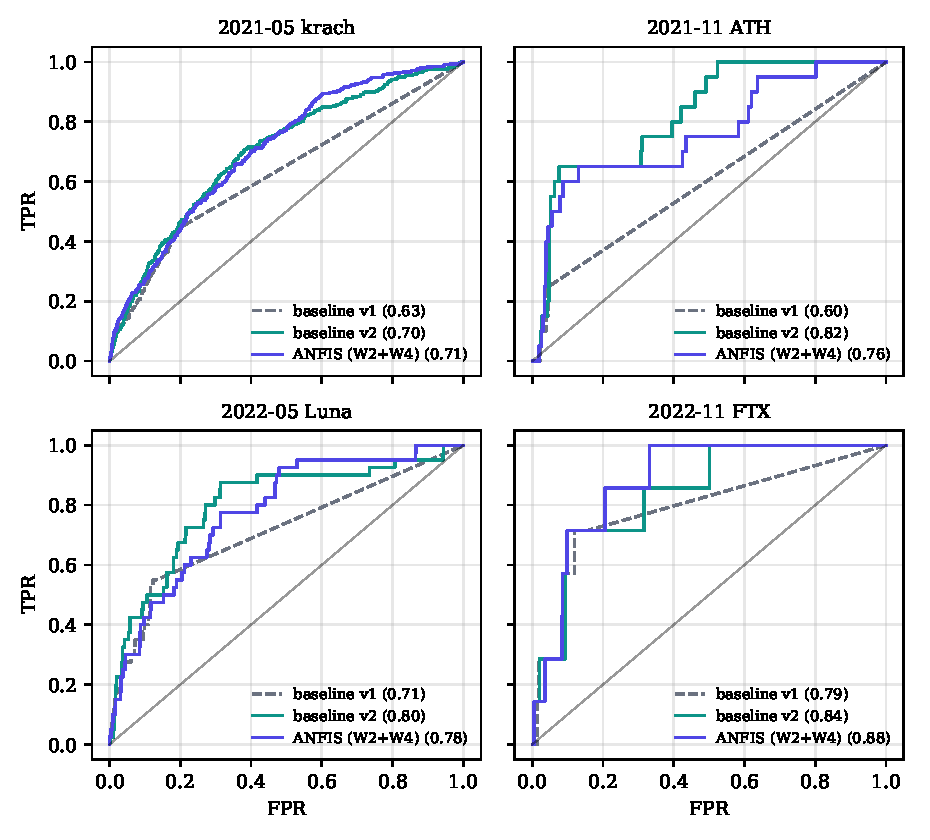
\includegraphics[width=.9\linewidth]{Images/roc-windows.pdf}
\caption{Krzywe ROC baseline~v1, baseline~v2 i~ANFIS W2+W4 w~podziale na okna (w~nawiasach AUC)}
\label{fig:rocwin}
\end{figure}

\paragraph{Wrażliwość na definicję populacji.} Populacja ewaluacji (ADR~0008) zawiera konsumpcje
w~bloku wykrycia ($k=0$), w~których stan puli na koniec bloku jest już stanem po konsumpcji, oraz
konsumpcje, przed którymi w~bloku $B+k$ inne transakcje zmieniły stan pul. Tabela~\ref{tab:sensitivity}
powtarza metryki dla trzech wariantów populacji: \emph{pełna} (jak w~tab.~\ref{tab:models}),
\emph{bez $k=0$} (bez konsumpcji atomowych w~bloku wykrycia) oraz \emph{bot pierwszy} (z~konsumpcji
\texttt{two\_pool} zostają tylko te z~$k\ge1$, w~których transakcja konsumująca była pierwszym swapem
bloku $B+k$ w~pulach pary; pozostałe konsumpcje \texttt{two\_pool} mają etykietę nieokreśloną i~są
wykluczone, negatywy pozostają bez zmian). W~wariantach \emph{pełna} i~\emph{bez $k=0$} kolejność
modeli według AUC jest identyczna. W~wariancie \emph{bot pierwszy} AUC każdego modelu rośnie,
najbardziej baseline~v2 (z~0,796 do 0,867), który wyprzedza wówczas ANFIS~W2+W4 (0,829); system
Mamdaniego pozostaje poniżej 0,5 w~każdym wariancie.

\begin{table}[H]\centering\footnotesize\setlength{\tabcolsep}{4pt}
\caption{Metryki modeli na wszystkich oknach łącznie dla trzech wariantów populacji ewaluacji
  (próg 50; AUC z~95\,\% CI z~bootstrapu)}\label{tab:sensitivity}
\begin{tabular}{llrrrl}
\toprule
Model & Wariant & $n$ & $n_+$ & PR-AUC & AUC [95\,\% CI] \\
\midrule
baseline v1   & pełna        & 4\,685 & 544 & 0{,}210 & 0{,}654 [0{,}63--0{,}68] \\
              & bez $k=0$    & 4\,561 & 423 & 0{,}177 & 0{,}664 [0{,}64--0{,}69] \\
              & bot pierwszy & 4\,290 & 156 & 0{,}107 & 0{,}756 [0{,}72--0{,}79] \\
\midrule
Mamdani       & pełna        & 4\,685 & 544 & 0{,}097 & 0{,}354 [0{,}33--0{,}38] \\
              & bez $k=0$    & 4\,561 & 423 & 0{,}079 & 0{,}362 [0{,}33--0{,}39] \\
              & bot pierwszy & 4\,290 & 156 & 0{,}035 & 0{,}410 [0{,}35--0{,}47] \\
\midrule
baseline v2   & pełna        & 4\,685 & 544 & 0{,}326 & 0{,}796 [0{,}78--0{,}81] \\
              & bez $k=0$    & 4\,561 & 423 & 0{,}283 & 0{,}808 [0{,}79--0{,}83] \\
              & bot pierwszy & 4\,290 & 156 & 0{,}171 & 0{,}867 [0{,}84--0{,}89] \\
\midrule
ANFIS W2      & pełna        & 4\,685 & 544 & 0{,}269 & 0{,}787 [0{,}77--0{,}81] \\
              & bez $k=0$    & 4\,561 & 423 & 0{,}221 & 0{,}788 [0{,}77--0{,}81] \\
              & bot pierwszy & 4\,290 & 156 & 0{,}107 & 0{,}795 [0{,}76--0{,}83] \\
\midrule
ANFIS W2+W4   & pełna        & 4\,685 & 544 & 0{,}369 & 0{,}818 [0{,}80--0{,}83] \\
              & bez $k=0$    & 4\,561 & 423 & 0{,}310 & 0{,}817 [0{,}80--0{,}84] \\
              & bot pierwszy & 4\,290 & 156 & 0{,}163 & 0{,}829 [0{,}79--0{,}86] \\
\bottomrule
\end{tabular}
\end{table}

\subsection{Stabilność modelu ANFIS}

Dla obu konfiguracji ANFIS powtórzono trening z~pięcioma ziarnami generatora (42--46), które
sterują podziałem walidacyjnym i~tasowaniem minipaczek; dane i~hiperparametry były identyczne.
Wyniki (rys.~\ref{fig:seeds}, \texttt{results/evaluation-seeds.csv}): konfiguracja W2 osiąga na
wszystkich oknach AUC $0{,}719 \pm 0{,}081$ (rozstęp od 0,584 do 0,787), a~konfiguracja W2+W4
$0{,}822 \pm 0{,}005$ (od 0,818 do 0,830). Odchylenie standardowe PR-AUC wynosi odpowiednio 0,070
i~0,004. Na oknie treningowym 2021-05 obie konfiguracje są stabilne (sd AUC 0,004 i~0,003);
rozrzut konfiguracji W2 pochodzi z~okien testowych 2022-05 (sd 0,062) i~2022-11 (sd 0,107).
Obie konfiguracje nie są jednak porównywane na równych warunkach. W2+W4 ma okno 2022-05
w~treningu, więc jej wynik na wszystkich oknach łączy dwa okna treningowe z~dwoma testowymi,
podczas gdy W2 ma jedno okno treningowe i~trzy testowe. Mniejszy rozrzut W2+W4 po części
bierze się właśnie stąd; miarodajne dla generalizacji są tylko okna 2021-11 i~2022-11.

\begin{figure}[H]\centering
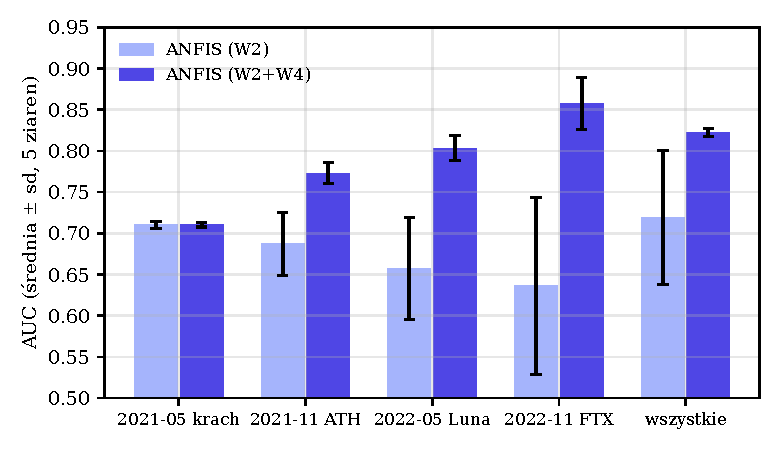
\includegraphics[width=.75\linewidth]{Images/seeds.pdf}
\caption{AUC ANFIS według okien: średnia i~odchylenie standardowe z~pięciu ziaren}
\label{fig:seeds}
\end{figure}

\subsection{Wstępna ocena ekonomiczna}

Tabela~\ref{tab:econ} charakteryzuje okazje od strony ekonomicznej: szacowany zysk brutto
z~optymalnej transakcji dwupulowej, wielkość tej transakcji, koszt gazu według założeń
baseline~v1 (220\,000 jednostek przy medianowej cenie gazu bloku) oraz udział okazji, dla których
szacowany zysk netto jest dodatni. Ostatnia kolumna podaje ten udział przy koszcie gazu
zmniejszonym o~połowę i~podwojonym, jako analizę wrażliwości na cenę gazu.

\begin{table}[H]\centering\footnotesize\setlength{\tabcolsep}{3pt}
\caption{Ekonomia okazji według okien (mediany; cztery pary łącznie). $\Pi$ --- szacowany zysk
  brutto, $\Delta y^{*}$ --- optymalna transakcja, $C_g$ --- koszt gazu wg baseline~v1;
  udział okazji z~$\Pi - C_g > 0$ przy $C_g$ oraz przy $0{,}5\,C_g$ / $2\,C_g$}\label{tab:econ}
\begin{tabular}{lrrrrrrrrr}
\toprule
Okno & $n$ & $S$ [\%] & gaz [gwei] & $\Pi$ [USD] & $\Pi_{p90}$ [USD] & $\Delta y^{*}$ [USD] & $C_g$ [USD] & $\Pi>C_g$ & $0{,}5\,C_g$ / $2\,C_g$ \\
\midrule
2021-05 krach & 2\,236 & 0{,}817 & 387 & 57{,}5 & 999 & 54\,592 & 200 & 27{,}0\,\% & 40{,}5 / 17{,}5\,\% \\
2021-11 ATH   & 891   & 0{,}698 & 136 & 11{,}2 & 67  & 23\,459 & 134 & 5{,}3\,\%  & 9{,}8 / 2{,}8\,\% \\
2022-05 Luna  & 1\,296 & 0{,}795 & 279 & 8{,}9  & 145 & 9\,231  & 118 & 14{,}7\,\% & 19{,}6 / 10{,}3\,\% \\
2022-11 FTX   & 406   & 0{,}758 & 70  & 2{,}5  & 44  & 3\,092  & 20  & 17{,}0\,\% & 24{,}6 / 11{,}3\,\% \\
\bottomrule
\end{tabular}
\end{table}

Dla konsumpcji atomowych o~trasie \texttt{two\_pool} można zestawić szacunek z~faktem
(tab.~\ref{tab:realized}). Mediana zysku zrealizowanego przez beneficjenta przewyższa medianę
szacowanego zysku brutto z~optymalnej transakcji dwupulowej we wszystkich oknach. Sama mediana
ilorazu tych wielkości (4,7 w~oknie 2021-05) niewiele jednak mówi, bo miesza konsumpcje o~różnym
opóźnieniu. Po rozbiciu według $k$ obraz jest inny. Dla $k=1$ (208 z~500 konsumpcji w~tym oknie)
mediana ilorazu wynosi 1,00, a~w~46\,\% przypadków fakt różni się od szacunku o~mniej niż
5\,\%: bot wykonał niemal dokładnie tę transakcję, którą system wyliczył ze stanu bloku. Dla
$k=0$ mediana sięga 19, bo stan na koniec bloku to już resztka po konsumpcji i~szacunek jest
z~definicji zaniżony. Dla $k=2$ i~$k=3$ mediana rośnie do 5 i~21: rozbieżność zdążyła się
powiększyć, zanim ktoś ją zamknął. Iloraz 4,7 jest więc wypadkową jednego przypadku, w~którym
szacunek trafia, i~trzech, w~których porównywany jest niewłaściwy stan puli.
O~wartości ilorazu rozstrzyga przy tym nie samo opóźnienie, lecz miejsce transakcji w~bloku.
Wśród konsumpcji par kwotowanych w~stablecoinie z~$k\ge1$ (410 we wszystkich oknach) transakcja
bota była pierwszym swapem bloku $B+k$ w~pulach pary w~163 przypadkach: mediana ilorazu wynosi tam
1,00 przy rozstępie międzykwartylowym 1,00--1,01, a~wielkość transakcji bota odpowiada optymalnej
transakcji wyliczonej przez system (mediana ilorazu 0,99). Dla pozostałych 247 konsumpcji,
w~których wcześniejsze swapy innych transakcji zmieniły stan pul, mediana ilorazu wynosi 9,64
(kwartyle 2,40 i~37,14), a~transakcja bota jest trzykrotnie większa od optymalnej dla stanu
z~bloku wykrycia.
Rzeczywiste zużycie gazu (mediana
142--155~tys. jednostek) jest niższe od założonych 220\,000, a~w~oknie 2021-05 131 z~618
konsumpcji atomowych ma zerową cenę gazu w~transakcji. Łączny zysk netto beneficjentów trzeba
sumować po transakcjach, nie po okazjach, bo jedna transakcja zamyka często rozbieżność widoczną
w~kilku kolejnych blokach. Za 570 konsumpcji \texttt{two\_pool} odpowiada 345 transakcji o~łącznym
zysku netto 1,15~mln USD, z~czego 1,13~mln USD przypada na okno 2021-05. Sumowanie po okazjach
dałoby 1,87~mln USD, czyli zawyżyłoby wynik o~ponad połowę.
Zestawienie szacunku netto baseline~v1 z~etykietą: spośród 544 okazji skonsumowanych z~zyskiem
299 miało szacowany zysk netto ujemny, a~spośród 840 okazji o~dodatnim szacunku netto 595 nie
zostało skonsumowanych z~zyskiem.

\begin{table}[H]\centering\scriptsize\setlength{\tabcolsep}{3.5pt}
\caption{Konsumpcje atomowe o~trasie \texttt{two\_pool}: szacunek a~fakt (mediany); $k=0$ ---
  udział konsumpcji w~bloku okazji}\label{tab:realized}
\begin{tabular}{lrrrrrrrr}
\toprule
Okno & $n$ & zysk zreal. [USD] & $\Pi$ szac. [USD] & iloraz & gaz zreal. [USD] & $C_g$ szac. [USD] & gaz [jedn.] & $k=0$ \\
\midrule
2021-05 krach & 500 & 1\,020 & 171 & 4{,}70 & 225 & 295 & 149\,531 & 23\,\% \\
2021-11 ATH   & 20  & 225    & 120 & 1{,}01 & 131 & 142 & 155\,402 & 0\,\% \\
2022-05 Luna  & 43  & 700    & 76  & 2{,}56 & 129 & 98  & 154\,361 & 21\,\% \\
2022-11 FTX   & 7   & 176    & 43  & 1{,}91 & 11  & 17  & 142\,587 & 14\,\% \\
\bottomrule
\end{tabular}
\end{table}

\subsection{Dyskusja wyników i~ograniczenia}

Wyniki układają się w~spójny obraz po ustaleniu, co mierzy etykieta. To tutaj zaczyna się
dyskusja, a~kończy ją lista ograniczeń systemu.

\paragraph{Co mierzy etykieta?} Etykieta pozytywna oznacza, że okazja została skonsumowana
transakcją atomową o~trasie dwupulowej i~beneficjent na niej zarobił. 544 z~570 skonsumowanych
okazji były zyskowne, więc jest ona w~praktyce równoważna stwierdzeniu ,,ktoś to wziął''. Zatem
można stwierdzić, że modele oceniane na tej populacji przewidują zachowanie konkurencji, a~nie
wykonalność okazji arbitrażowej dla zewnętrznego obserwatora. Ta różnica tłumaczy trzy
obserwacje: odwrócenie systemu Mamdaniego, kalibrację baseline~v2 i~granicę, na której zatrzymał
się ANFIS.

\paragraph{Modele.} System Mamdaniego działa odwrotnie do etykiety: jego reguły odpowiadają na
pytanie ,,czy ja zdążę i~na tym zarobię''. Karzą wysoki koszt gazu i~dużą aktywność w~bloku,
tymczasem okazje skonsumowane w~oknie 2021-05 miały wyższą medianę $G$ i~$M$ niż pozostałe, bo
wysoki ruch w~bloku świadczy o~wysokiej obecności botów. Term ,,zaporowy'' dla $G$ spełnia
1,2\,\% bloków w~oknie 2021-05 i~żaden blok w~oknach z~2022~roku. Reguła wetująca dla gazu
praktycznie się nie uruchamia. Dla trzech z~czterech par cecha $L$ wynosi 100 w~każdym bloku
z~okna 2021-05, więc term ,,głęboka'' jest zawsze spełniony i~$L$ nie różnicuje okazji.
Kalibracja baseline~v2 wyzerowała wagę kosztu gazu i~sprowadziła model do rankingu po zysku
brutto. ANFIS uczony na tych samych danych osiągnął AUC 0,818 w~porównaniu do 0,796 dla
baseline~v2, przy nakładających się przedziałach ufności. Przy progu 50 oznacza on jako pozytywne
58--70\,\% okazji. Uczenie z~danych odzyskało ranking po wielkości okazji i~niewiele ponad to.

\paragraph{Szacunek a~fakt.} Mediana ilorazu zysku zrealizowanego do szacowanego, wynosząca 4,7
w~oknie 2021-05, jest wynikiem mieszania konsumpcji o~różnym opóźnieniu i~różnym miejscu
w~bloku. W~podzbiorze opisanym w~podrozdziale~4.7, gdy transakcja bota była pierwszym swapem
bloku, mediana ilorazu wynosi 1,00 przy rozstępie międzykwartylowym 1,00--1,01, a~dla pozostałych
konsumpcji 9,64, ponieważ między wykryciem a~konsumpcją cudze transakcje zmieniły stan pul.
Arytmetyka AMM o~stałym iloczynie odtwarza więc zysk co do wartości, a~rozjazd bierze się z~czasu.
Statystyki ekonomiczne liczone po okazjach zawyżają wynik, bo 570 konsumpcji dwupulowych to 345
transakcji: suma po transakcjach daje 1,15~mln USD zamiast 1,87~mln USD.

\paragraph{Statystyka.} Klasa pozytywna skupia się w~oknie 2021-05 (477 z~544), a~w~oknach 3--5
liczy 20, 40 i~7 przypadków. Stąd przedziały ufności szerokości do ponad 0,3, a~AUC 0,879 przy
siedmiu pozytywach jest liczbą, której nie należy interpretować. Wiersz ,,wszystkie okna'' miesza
rozpoznawanie okna z~rozpoznawaniem okazji, bo udział pozytywów wynosi 22\,\% w~oknie 2021-05
i~1,7--3,1\,\% w~pozostałych; zawiera też dane treningowe (45,2\,\% populacji dla baseline~v2
i~ANFIS~W2, 72,5\,\% dla W2+W4). Porównania modeli są wiarygodne tylko w~podziale na okna
testowe. Wynik ziarna 42 w~tabeli głównej jest dla ANFIS~W2 górnym krańcem rozstępu
(0,787 z~0,584--0,787), a~dla W2+W4 dolnym (0,818 z~0,818--0,830), więc tabela pokazuje
konfigurację W2 od najlepszej strony. Analiza wrażliwości na definicję populacji zachowuje ranking
między wariantami ,,pełna'' i~,,bez $k=0$''; w~wariancie ,,bot pierwszy'' baseline~v2 (0,867)
wyprzedza ANFIS~W2+W4 (0,829), a~system Mamdaniego pozostaje poniżej 0,5 (0,410).

\paragraph{Ograniczenia.} System obejmuje wyłącznie arbitraż dwupulowy między giełdami
Uniswap~V2 i~Sushiswap, więc 144 konsumpcje o~trasie wielopulowej, czyli co piąta konsumpcja
atomowa, mają etykietę nieokreśloną. Okno 2021-05 poprzedza nowy system opłat transakcyjnych
w~sieci Ethereum (EIP-1559), a~trzy pozostałe następują po nim, więc ewaluacja łączy dwa reżimy
opłat, a~cecha $G$ nie jest między nimi w~pełni porównywalna. Heurystyki beneficjenta i~trasy
przenoszą swoje błędy wprost na etykiety, a~kontrola ręczna objęła 13 przypadków. Cecha $M$
narusza zasadę oceny ex~ante: korzysta z~percentyli liczonych po całym oknie, a~w~bloku wykrycia
obejmuje także swapy transakcji konsumującej. System nie symuluje wykonania transakcji, nie widzi
mempoola ani pakietów prywatnych, takich jak Flashbots. Model ANFIS jest uczony metodą Adam na
wszystkich parametrach, a~nie hybrydą z~estymacją najmniejszych kwadratów opisaną
w~rozdziale~2.4, więc wyniki nie przenoszą się wprost na klasyczny ANFIS. Wnioski obowiązują
w~granicach danych: cztery pary, dwie giełdy i~cztery dwutygodniowe okna.
